\section{Multi-fidelity-surrogate nonlinear ROM}\label{sec:vf-mfs}

\subsection*{Concept and purpose}

\citet{he2023mfsnlrom} build a multi-fidelity-surrogate nonlinear reduced-order model (MFS-NLROM) of a geometrically nonlinear structure from a small number of static nonlinear solves. The reduced equilibrium of a modal model contains one purely nonlinear term, the projected internal force with its linear part removed. The paper's observation is that the \emph{linear} modal displacement under the same load is available in closed form (one matrix--vector product), so it can serve as a cheap, low-fidelity input from which the nonlinear force is regressed. The nonlinear modal displacement then follows from a relation that needs no Newton iteration. The method is tested on a clamped beam and on a tapered wing cantilever, in statics, free decay and as a backbone curve, and against a polynomial baseline, the implicit condensation and expansion (ICE) model of \Cref{sec:vf-ice}.

In the packages the study uses \anchor{fea_engine.elements.Beam2DCorotational} for the beam, \anchor{fea_engine.elements.Shell4Director} (a director-based total-Lagrangian shell) and the total-Lagrangian ten-node tetrahedron for the wing, and \rom{} for the surrogate, the polynomial baseline, the Newmark integrator for reduced models and the harmonic-balance backbone solver \anchor{rom_engine.solve_nnm_backbone}. The study tests three things: that the relation below holds on a beam whose answer is checked against an exact benchmark, that the surrogate generalises inside its training range, and that the backbone computed by harmonic balance on the reduced model agrees with free vibration of the full model.

\subsection*{Mathematics as implemented}

The full-order model is
\begin{equation}\label{eq:mfs-fom}
\mathbf M\ddot{\mathbf u}+\mathbf C\dot{\mathbf u}+\mathbf f_{\rm int}(\mathbf u)=\mathbf F(t),
\end{equation}
with the linear modes $(\mathbf K-\lambda_r\mathbf M)\boldsymbol\phi_r=\mathbf 0$ mass-normalised, $\mathbf u\approx\boldsymbol\Phi\mathbf q$ and $\boldsymbol\Lambda=\operatorname{diag}(\lambda_r)$. Projecting the static form onto the retained modes and separating the linear part of the internal force defines the nonlinear modal force $\mathbf F_{\rm nl}$:
\begin{equation}\label{eq:mfs-nl}
\boldsymbol\Lambda\,\mathbf q_{\rm nl}+\mathbf F_{\rm nl}=\boldsymbol\Phi^{T}\mathbf F,\qquad
\boldsymbol\Lambda\,\mathbf q_{\rm l}=\boldsymbol\Phi^{T}\mathbf F .
\end{equation}
Subtracting the two equations gives the multi-fidelity relation
\begin{equation}\label{eq:mfs-mf}
\boxed{\;\mathbf q_{\rm nl}=\mathbf q_{\rm l}-\boldsymbol\Lambda^{-1}\mathbf F_{\rm nl}\;},\qquad \mathbf F_{\rm nl}=\mathbf f(\mathbf q_{\rm l}),
\end{equation}
where the surrogate $\mathbf f$ takes the linear modal displacement $\mathbf q_{\rm l}$, known at run time, as input. Each component is a radial-basis-function expansion over the $N$ training samples $\mathbf q_{\rm l}^{(m)}$,
\begin{equation}\label{eq:mfs-rbf}
F_{{\rm nl},i}(\mathbf q_{\rm l})=\sum_{m=1}^{N}w^{(i)}_m\,\psi\!\left(\lVert\mathbf q_{\rm l}-\mathbf q_{\rm l}^{(m)}\rVert\right),
\end{equation}
with the kernels $\psi(r)=\sqrt{r^2+c^2}$ (multiquadric, MQ), $r^3$ (cubic), $r^2\ln r$ (thin-plate spline, TPS) and $e^{-r^2/c^2}$ (Gaussian). The baseline instead regresses $\mathbf F_{\rm nl}$ against the \emph{nonlinear} displacement with the quadratic-plus-cubic form
\begin{equation}\label{eq:mfs-ice}
F_{{\rm nl},i}=\sum_{j\le k}A^{(i)}_{jk}q_jq_k+\sum_{j\le k\le l}B^{(i)}_{jkl}q_jq_kq_l ,
\end{equation}
whose argument is the unknown, so it needs a Newton solve of an $n\times n$ system at each step.

\emph{Training.} Loads are drawn by optimal Latin-hypercube sampling (OLHS) over modal force amplitudes, scaled so that the peak shape component of each mode reaches a target multiple of the thickness. For each load one nonlinear static solve returns $\mathbf q_{\rm nl}$ and $\mathbf F_{\rm nl}=\boldsymbol\Phi^{T}\mathbf F-\boldsymbol\Lambda\mathbf q_{\rm nl}$.

\emph{Dynamics.} With Rayleigh damping the reduced equation is
\begin{equation}\label{eq:mfs-dyn}
\ddot{\mathbf q}_{\rm nl}+\mathbf C_m\dot{\mathbf q}_{\rm nl}+\boldsymbol\Lambda\mathbf q_{\rm nl}+\mathbf F_{\rm nl}(\mathbf q_{\rm l})=\boldsymbol\Phi^{T}\mathbf F(t),
\end{equation}
integrated by Newmark-$\beta$ ($\beta=\tfrac14$, $\gamma=\tfrac12$). Three treatments of the implicit force were compared: \texttt{newton} solves $\mathbf q_{\rm l}=\mathbf q_{\rm nl}+\boldsymbol\Lambda^{-1}\mathbf F_{\rm nl}(\mathbf q_{\rm l})$ exactly at each step; \texttt{fixed\_point} uses a lagged force with one Picard refinement; \texttt{sign\_deviation} is the predictor--corrector scheme reconstructed from the publication's equations.

\emph{Backbone.} The frequency of the nonlinear normal mode as a function of amplitude is computed for the reduced models by harmonic balance with five harmonics and continuation. The full-order reference is undamped free vibration released from static equilibria, with the period measured.

\emph{Metric.} The accuracy of a prediction $\hat y$ against the reference $y$ is the coefficient of determination
\begin{equation}\label{eq:mfs-r2}
R^2=1-\frac{\sum_k(y_k-\hat y_k)^2}{\sum_k(y_k-\bar y)^2}.
\end{equation}

\subsection*{Geometry and mesh}

\Cref{fig:vf-mfs-geom} shows the two structures and \Cref{tab:vf-mfs-setup} their set-up. The beam is the clamped--clamped flat beam of the publication, meshed with 40 corotational beam elements (117 free degrees of freedom). The publication gives the wing only as a dimensioned schematic whose four labelled in-plane edges cannot close a quadrilateral (280 mm exceeds $50+60+16$ mm); digitising the schematic gives the pentagon of \Cref{fig:vf-mfs-geom}b, a taper from a 16~mm chord to a 50~mm chord over 220~mm of span followed by a constant 50~mm cap, clamped at the 50~mm end. The wing is 1.15~mm thick, so its aspect ratio is high; this decides which element models it.

\begin{figure}[tbp]
\centering
\includegraphics[width=0.98\linewidth]{figures/ch14_geom_mfs.pdf}
\caption{Structures of the multi-fidelity study, drawn from the dimensions of the report. (a) Flat beam with its 40 elements and the uniform pressure of the static sweep. (b) Wing planform reconstructed from the publication's schematic; the shell model of this planform (140 elements) is the reference of the wing results.}\label{fig:vf-mfs-geom}
\end{figure}

\begin{table}[tbp]
\centering\footnotesize
\caption{Set-up of the multi-fidelity study. ``Assumed'' marks a value the publication does not give.}\label{tab:vf-mfs-setup}
\begin{tabularx}{\linewidth}{@{}>{\raggedright\arraybackslash}p{3.0cm} >{\raggedright\arraybackslash}X >{\raggedright\arraybackslash}X@{}}
\toprule
Item & Flat beam & Wing (shell reference)\\
\midrule
Dimensions & $228.6\times12.7\times0.787$ mm & span 280 mm, chord 16--50 mm, thickness 1.15 mm\\
Material & $E=204.8$ GPa, $\rho=7870$ kg/m$^3$ & T7050: $E=70.3$ GPa, $\rho=2830$ kg/m$^3$, $\nu=0.33$\\
Element, mesh & \texttt{Beam2DCorotational}, 40 elements, 117 free dofs & \texttt{Shell4Director}, 140 elements\\
Boundary & clamped--clamped & clamped at the 50 mm end\\
Retained modes & 1, 3, 5 (the symmetric ones) & 3 (16.67, 83.14, 218.36 Hz)\\
Training / test samples & 30 / 21 (publication: same) & 30 / 15 (publication: 800 / 400, 20 modes)\\
Damping & 1\,\% modal Rayleigh at modes 1 and 5 (assumed) & 1\,\% at modes 1 and 3 (assumed)\\
Load & uniform pressure, $\pm2000$ Pa & tip load, up to about 46 mm tip displacement\\
\bottomrule
\end{tabularx}
\end{table}

The retained modes of the beam are 1, 3 and 5 and not 1, 2 and 3, because a symmetric load on a symmetric clamped beam excites only the symmetric modes. The training and test sizes of the wing are far below the publication's, which a nonlinear shell model of this size cannot supply on the available machines; three modes matches the publication's own three-order modal-force training basis.

\subsection*{Results: flat beam}

\emph{Modes.} \Cref{tab:vf-mfs-modes} compares the four lowest frequencies with the publication and with the closed-form Euler--Bernoulli result $\omega_n=(\beta_nL)^2\sqrt{EI/(\rho AL^4)}$. All differences are within the integer-hertz rounding of the publication, and the finite element model agrees with the closed form to $0.01\,\%$.

\begin{table}[tbp]
\centering\footnotesize
\caption{Linear frequencies of the clamped beam.}\label{tab:vf-mfs-modes}
\begin{tabular}{@{}rrrrr@{}}
\toprule
Mode & Publication (Hz) & This work (Hz) & Closed form (Hz) & Difference to publication\\
\midrule
1 & 79 & 78.97 & 78.97 & $-0.04\,\%$\\
2 & 218 & 217.68 & 217.68 & $-0.15\,\%$\\
3 & 427 & 426.75 & 426.74 & $-0.06\,\%$\\
4 & 706 & 705.44 & 705.43 & $-0.08\,\%$\\
\bottomrule
\end{tabular}
\end{table}

\emph{Nonlinear modal force and static accuracy.} The surfaces of the fitted force over the plane of the first two retained linear amplitudes (\Cref{fig:vf-mfs-surf}) have the axis ranges and the saddle shape of the publication's figure; its own training points and confidence-interval method are not published, so values cannot be matched point for point. \Cref{tab:vf-mfs-static} gives the static accuracy by kernel. The multiquadric kernel and the polynomial baseline agree with the publication; the ranking of the other three kernels differs, as expected with a different training set. Over the pressure sweep of \Cref{fig:vf-mfs}a both models agree with nonlinear finite elements to $R^2=1.0000$; the surrogate costs $0.05$~ms per case against $2.4$~ms for the baseline and $843$~ms for finite elements, a ratio of about $1.7\times10^{4}$ to the finite element solve (the order of the publication's table, with a machine-dependent absolute value).

\begin{figure}[tbp]
\centering
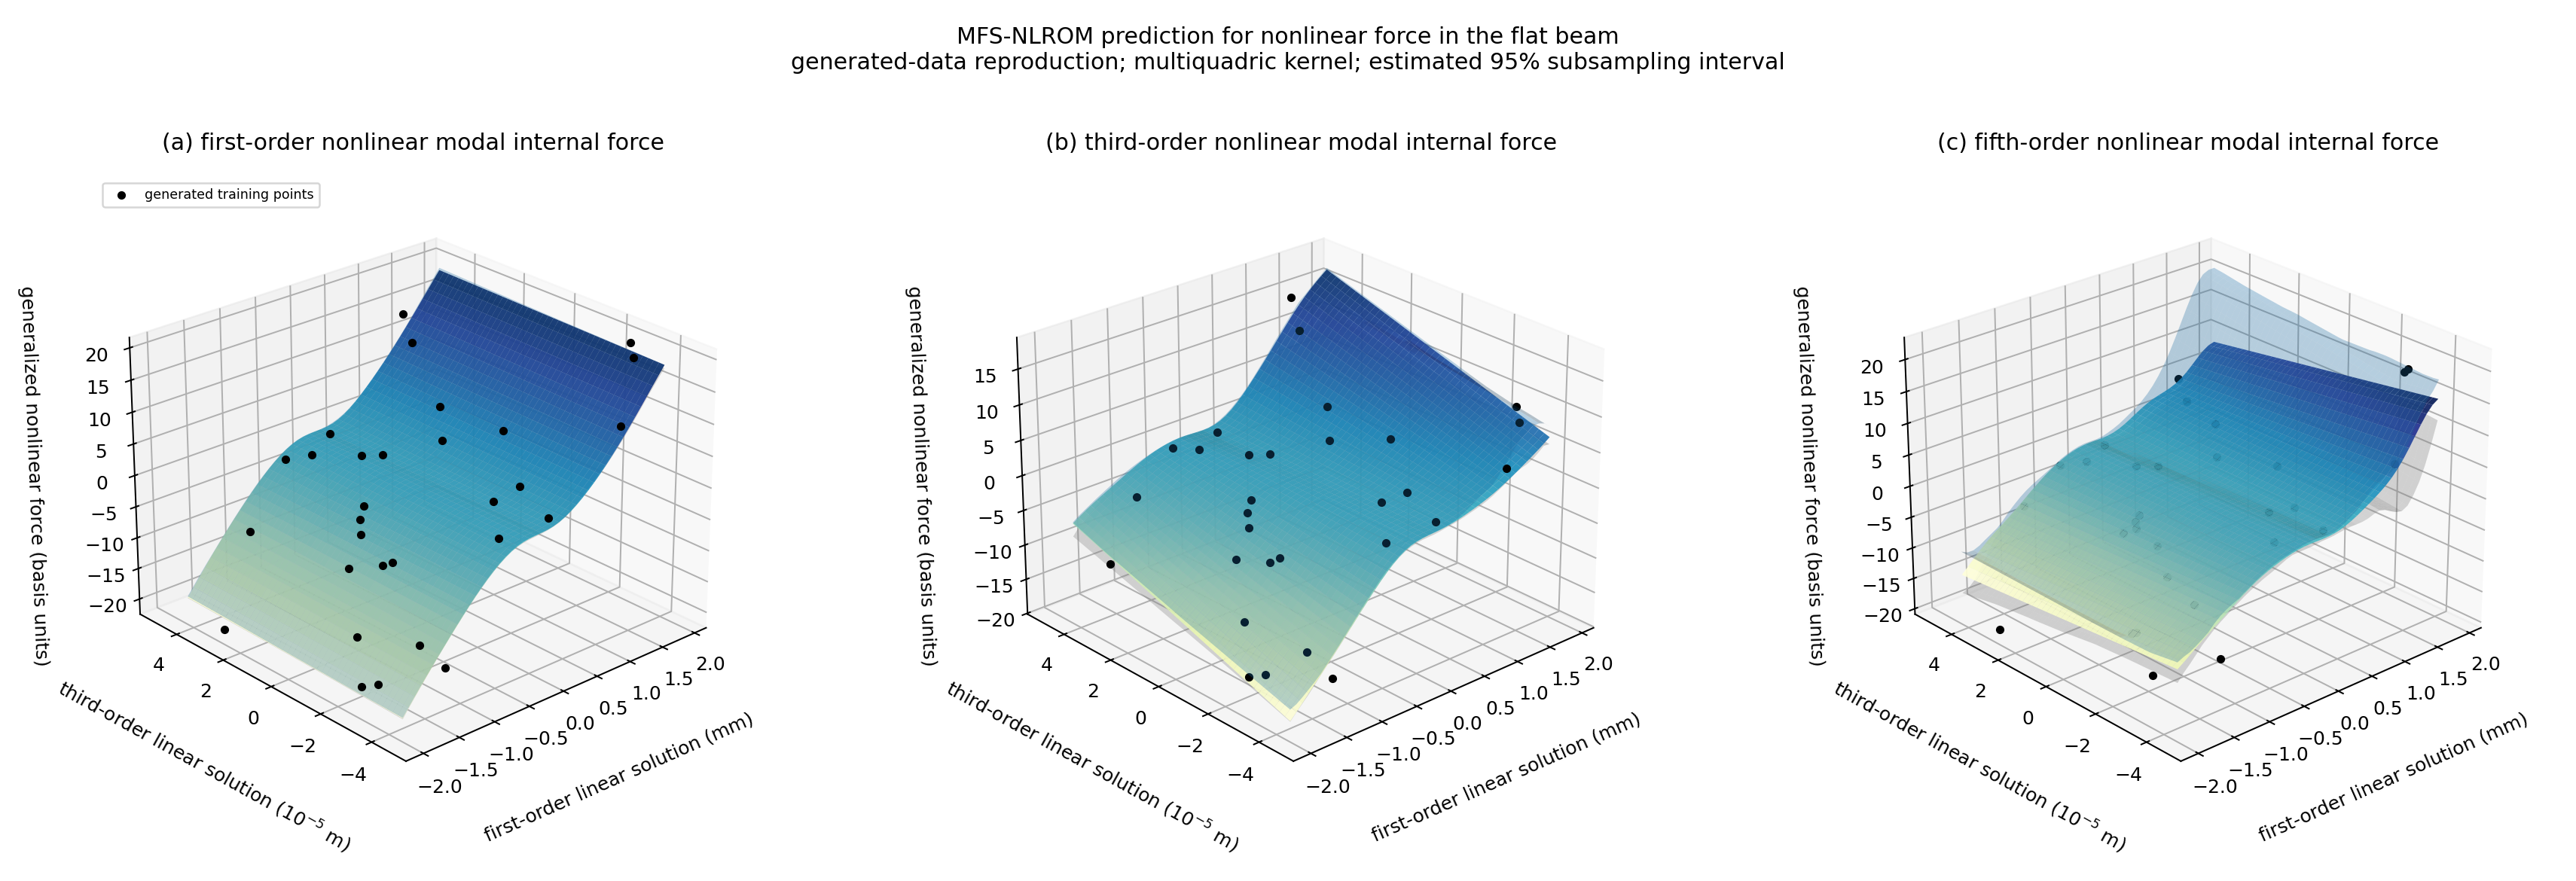
\includegraphics[width=0.8\linewidth]{figures/ch14r/mfs_surfaces.png}
\caption{Fitted nonlinear modal force of modes 1, 3 and 5 (multiquadric kernel) over the linear amplitudes of modes 1 and 3; the black dots are the OLHS training points of this run, and the shaded band is an improvised $95\,\%$ subsampling interval. The mode-5 input is held at its training mean. Plot of the reproduction report.}\label{fig:vf-mfs-surf}
\end{figure}

\begin{table}[tbp]
\centering\footnotesize
\caption{Static accuracy ($R^2$ against nonlinear finite elements, held-out samples) of the flat beam.}\label{tab:vf-mfs-static}
\begin{tabular}{@{}lrr@{}}
\toprule
Model & This work & Publication\\
\midrule
Multi-fidelity, multiquadric & 0.9982 & 0.9997\\
Multi-fidelity, cubic & 0.9889 & 0.9996\\
Multi-fidelity, thin-plate spline & 0.9860 & 0.9998\\
Multi-fidelity, Gaussian & 0.9968 & 0.9853\\
ICE polynomial & 1.0000 & 1.0000\\
\bottomrule
\end{tabular}
\end{table}

\emph{Free decay.} \Cref{tab:vf-mfs-decay} compares the tip response over 190~ms for two initial conditions: case~(a) releases the beam from the static state of the strongest negative load ($q_{\rm nl}/q_{\rm l}\approx0.5$, strongly hardening); case~(b) starts from half a thickness of the first mode shape. The Newton treatment of the implicit force and the polynomial baseline lie on the full-order curve (\Cref{fig:vf-mfs}b). The lagged-force path of the library translates the initial condition from $q_{\rm nl}$ to $q_{\rm l}$ with a single Picard refinement and lands $23\,\%$ short in case~(a), which gives $R^2<0$; the Newton path corrects this exactly. The reconstructed predictor--corrector scheme diverges in both cases.

\begin{table}[tbp]
\centering\footnotesize
\setlength{\tabcolsep}{4pt}
\caption{Free-decay accuracy ($R^2$ of the tip response against nonlinear finite elements), flat beam.}\label{tab:vf-mfs-decay}
\begin{tabular}{@{}lrrrrr@{}}
\toprule
Case & MFS, Newton & ICE & MFS, lagged force & MFS, predictor--corrector & Publication (MFS / ICE)\\
\midrule
(a) $F_{\rm nl}(0)=-2068$ Pa & 0.9971 & 0.9981 & $-0.89$ & $-853$ & 0.9837 / $-0.63$\\
(b) $q_{\rm nl}(0)=0.5\,t\,\phi_1$ & 0.9898 & 0.9987 & 0.9907 & $-3141$ & 0.9836 / 0.9008\\
\bottomrule
\end{tabular}
\end{table}

\emph{Sample size.} The held-out $R^2$ against the number of training samples (\Cref{fig:vf-mfs-samples}) is $0.844$, $0.986$, $0.9994$ and $1.0000$ for $N=9$, $15$, $30$ and $60$: substantial improvement at small $N$, and a knee near the publication's recommended $N=10n$.

\begin{figure}[tbp]
\centering
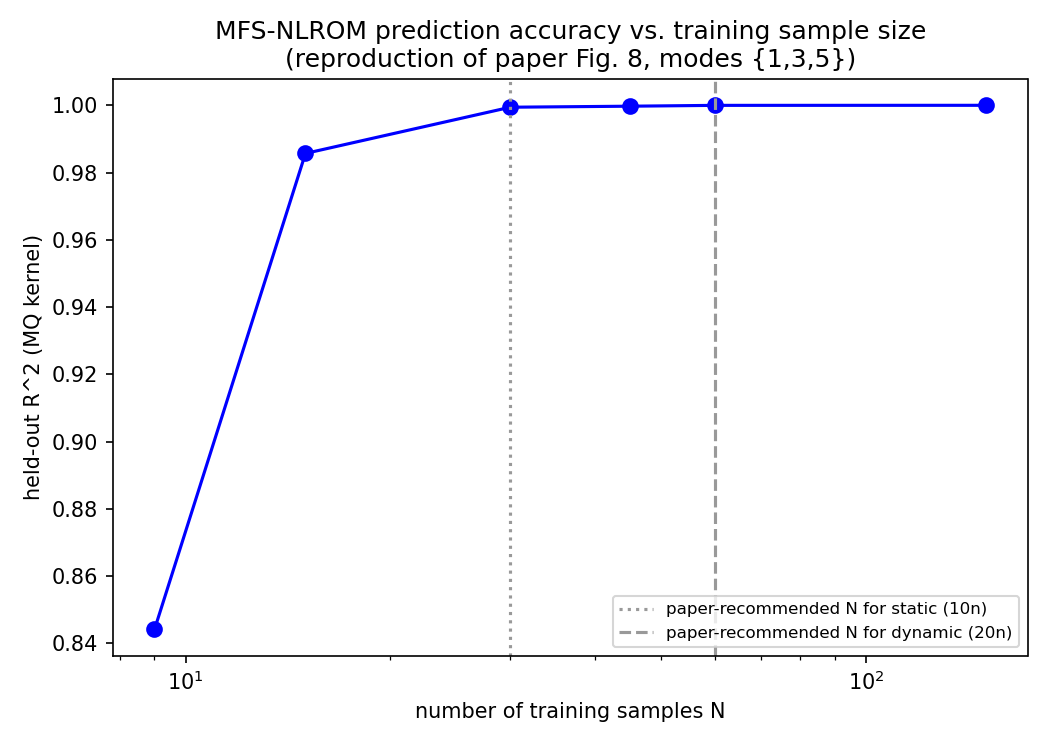
\includegraphics[width=0.6\linewidth]{figures/ch14r/mfs_samples.png}
\caption{Held-out $R^2$ against the number of training samples, flat beam. Plot of the reproduction report.}\label{fig:vf-mfs-samples}
\end{figure}

\begin{figure}[tbp]
\centering
\includegraphics[width=1.0\linewidth]{figures/ch14_mfs.pdf}
\caption{Flat beam of \citet{he2023mfsnlrom}. (a) Centre displacement over $\pm2000$~Pa: nonlinear FE, multi-fidelity surrogate and ICE ($R^2=\cvfMfsRtwoMfs$ and $\cvfMfsRtwoIce$ against FE). (b) Free decay of the first modal coordinate ($R^2=\cvfMfsDecayA$ for case a and $\cvfMfsDecayB$ for case b). (c) Backbone by harmonic balance against FE free vibration; largest frequency error $\cvfMfsBackErr$ over a hardening of $\cvfMfsHardening$ above the linear frequency. One surrogate evaluation takes \cvfMfsTmfs{}~s against \cvfMfsTfe{}~s for FE, a ratio of \cvfMfsSpeed.}\label{fig:vf-mfs}
\end{figure}

\emph{Backbone.} \Cref{tab:vf-mfs-back} gives the frequency of the first nonlinear mode against its amplitude. The beam hardens by about $22\,\%$ over the range; the largest error against free vibration of the full model is $0.96\,\%$ for the surrogate and $0.87\,\%$ for the baseline.

\begin{table}[tbp]
\centering\footnotesize
\caption{Backbone of the flat beam; linear frequency 78.97~Hz.}\label{tab:vf-mfs-back}
\begin{tabular}{@{}lrrrrrr@{}}
\toprule
$q_1$ ($\times10^{-5}$) & 2.05 & 2.96 & 3.86 & 4.76 & 5.67 & 6.57\\
\midrule
FE free vibration (Hz) & 80.56 & 83.08 & 85.96 & 88.50 & 93.00 & 96.27\\
MFS-NLROM (Hz) & 81.33 & 83.22 & 85.86 & 89.14 & 92.94 & 97.18\\
ICE (Hz) & 80.96 & 83.04 & 85.76 & 89.07 & 92.87 & 97.10\\
\bottomrule
\end{tabular}
\end{table}

\subsection*{Results: wing}

\emph{Reconstructed geometry and modes.} The first four frequencies of the reconstructed wing are 16.8, 84.0, 221.8 and 256.4~Hz with ten-node tetrahedra and 16.7, 83.0, 216.7 and 251.6~Hz with twenty-node hexahedra, against 15, 73, 191 and 223~Hz in the publication (\Cref{fig:vf-mfs-wing}a). The two meshes agree to $1$--$2\,\%$ on every mode, which is an independent confirmation of the converged answer. Clamping at the 50~mm end matches the publication to within $11$--$16\,\%$ uniformly on every mode, whereas clamping at the other end gives a ragged $7$--$45\,\%$ spread; a uniform spread is the signature of the right boundary condition, although it does not prove the publication's fixture, and the remaining gap is plausibly root-fixture stiffness that the schematic cannot specify.

\emph{Why the shell is the reference.} The wing is 1.15~mm thick and the solid model has one element layer through that thickness at an in-plane size of 90~mm, an aspect ratio near 78:1. The Green--Lagrange strain
\begin{equation}\label{eq:mfs-gl}
\mathbf E=\tfrac12\left(\nabla\mathbf u+\nabla\mathbf u^{T}+\nabla\mathbf u^{T}\nabla\mathbf u\right)
\end{equation}
is quadratic in displacement \emph{gradients}, and gradients across the thin layer are amplified: for the softest eigenmode the nonlinear internal force exceeds the linear prediction by a factor of 70 at 1~\textmu m of displacement (a rotation of about $0.0004^\circ$), scaling as $u^2$ against the linear term's $u^1$. A too-large load or time increment, rounding from the mesh condition number (about $2\times10^{11}$) and genuine large-rotation physics were each ruled out by direct tests; in-plane refinement barely changes the effect, and more layers through the thickness make it worse ($3957\times$ to $7128\times$ from one to four layers). A shell element never discretises the thickness, and its force ratio stays flat over six orders of magnitude of amplitude.

The choice of shell element matters as well. \Cref{tab:vf-mfs-shell} shows the ratio $q_{{\rm nl},1}/q_{{\rm l},1}$ for pure mode-1 loads (1 means no nonlinearity): the corotational shell shows no geometric stiffening even at a tip displacement of 46~mm, so an early run that used it fitted numerical noise and had a deeply negative held-out $R^2$; \texttt{Shell4Director} stiffens as it should and is the reference.

\begin{table}[tbp]
\centering\footnotesize
\caption{Ratio $q_{{\rm nl},1}/q_{{\rm l},1}$ for mode-1 tip loads of a given multiple of the thickness.}\label{tab:vf-mfs-shell}
\begin{tabular}{@{}lrrrr@{}}
\toprule
Tip load (thickness) & 3 & 10 & 20 & 40\\
\midrule
\texttt{Shell4MITCCorotational} & 1.00000 & 1.00000 & 0.99998 & 0.99992\\
\texttt{Shell4Director} & 0.99976 & 0.99765 & 0.99100 & 0.96780\\
\bottomrule
\end{tabular}
\end{table}

\begin{figure}[tbp]
\centering
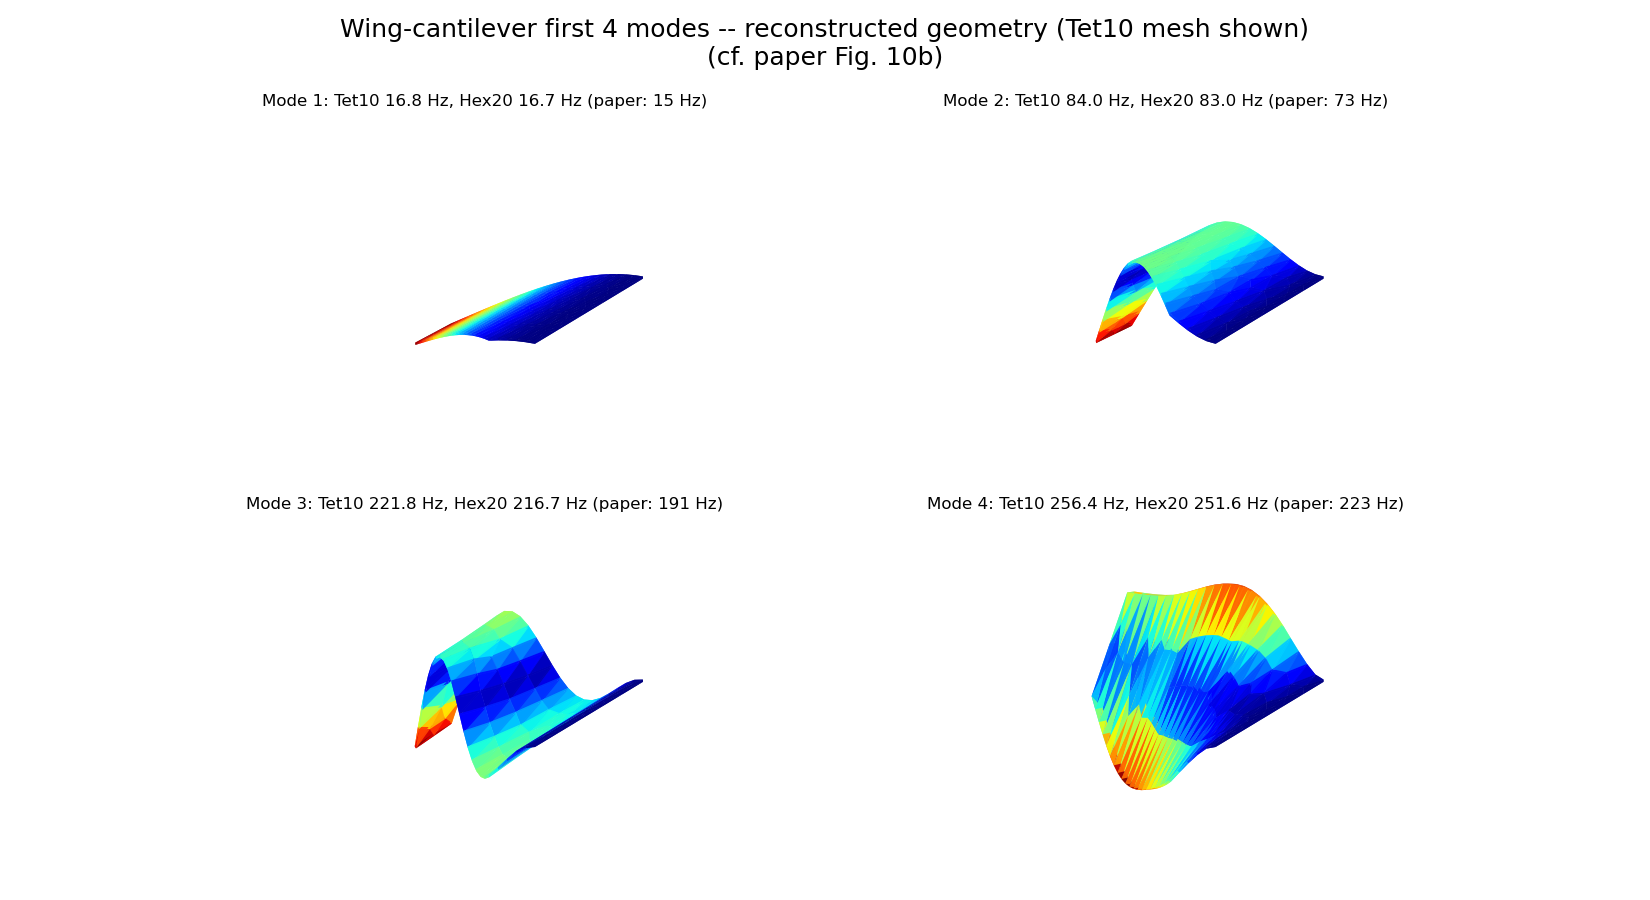
\includegraphics[width=0.8\linewidth]{figures/ch14r/mfs_wing_modes.png}
\caption{First four modes of the reconstructed wing (ten-node tetrahedron mesh; colour is displacement magnitude). Plot of the reproduction report.}\label{fig:vf-mfs-wing}
\end{figure}

\emph{Static tip sweep.} \Cref{fig:vf-mfs-wing2} (left) shows the tip displacement against the mode-1 linear amplitude. Both reduced models give a sweep $R^2$ of $1.0000$, but the nonlinear part is only $2.6$--$3.8\,\%$ of the linear modal force at these amplitudes and the linear finite element alone scores $0.9993$, so the discriminating number is the $R^2$ of the nonlinear deviation $w-w_{\rm lin}$: $0.984$ for the surrogate (Gaussian kernel, held-out force $R^2=0.974$; MQ $0.915$, cubic $0.909$, TPS $0.875$) and $0.9999$ for the polynomial baseline (held-out $0.997$). The polynomial wins because the true force is close to the quadratic-plus-cubic form it assumes; the surrogate shows a $-0.09$~mm zero-load offset from the Gaussian fit.

\begin{figure}[tbp]
\centering
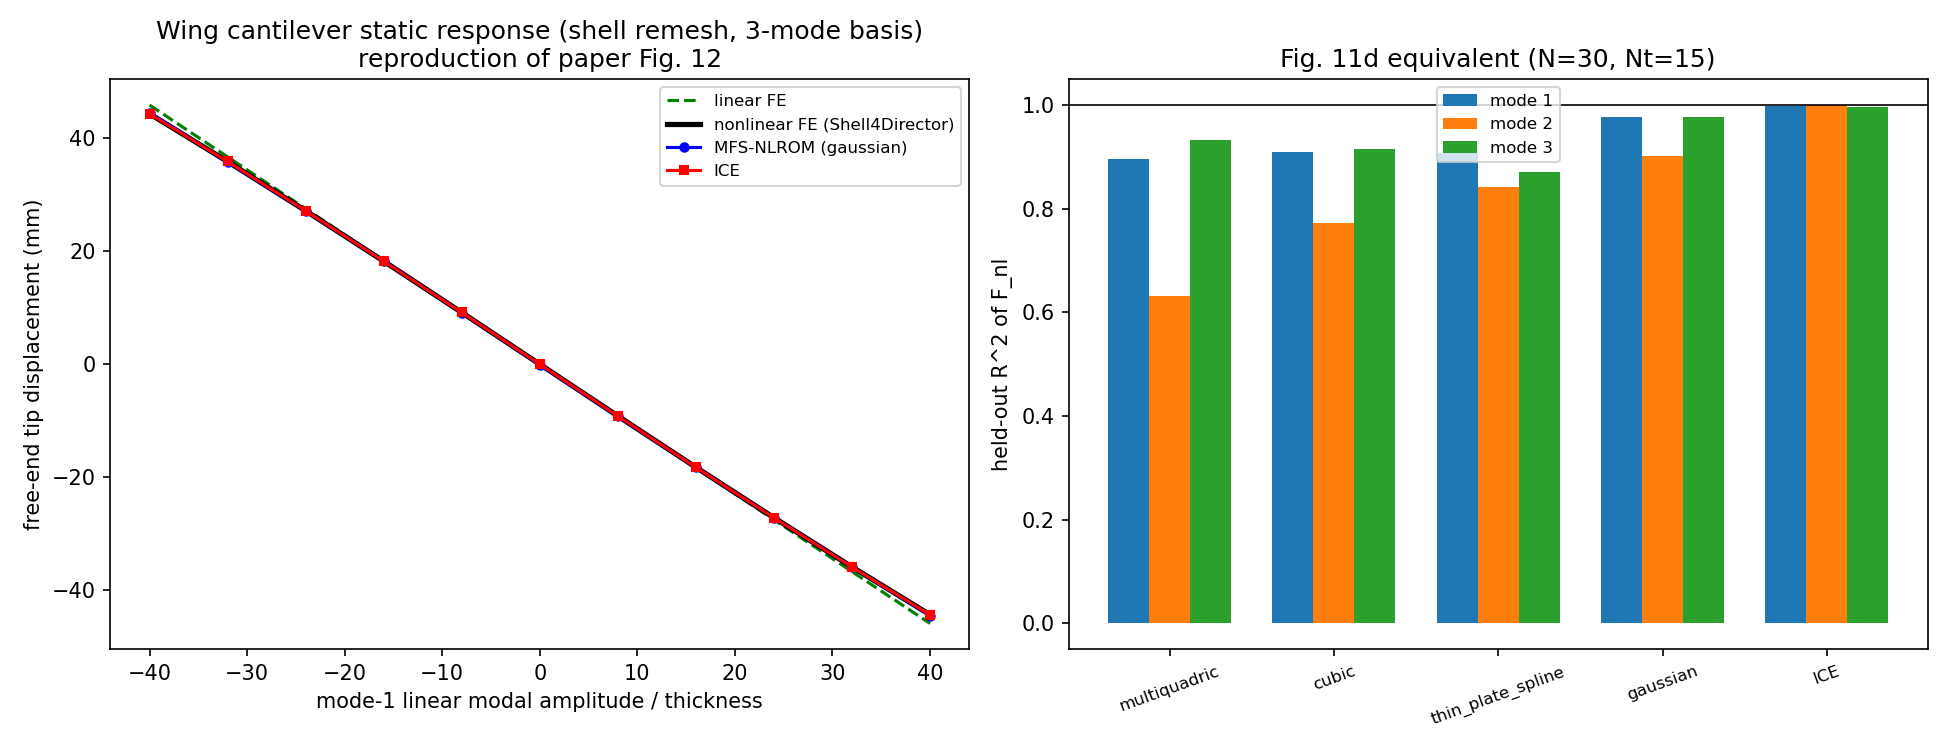
\includegraphics[width=0.8\linewidth]{figures/ch14r/mfs_wing_sweep.png}
\caption{Shell wing, static tip-load sweep. Left: tip displacement against the mode-1 linear amplitude for nonlinear FE, linear FE, MFS-NLROM (Gaussian) and ICE. Right: held-out $R^2$ of $F_{\rm nl}$ per mode and kernel. Plot of the reproduction report.}\label{fig:vf-mfs-wing2}
\end{figure}

\emph{Free decay.} \Cref{tab:vf-mfs-wdecay} gives the shell wing's tip response over about two periods ($\Delta t=2$~ms, 60 steps, about 22~mm amplitude). Case~(b) is an impulsive start with a mode-1 velocity and zero displacement, because a mode-shape displacement is not an admissible initial condition for a Green--Lagrange shell at this amplitude. Every scheme reaches $R^2\ge0.9998$, including the predictor--corrector that diverged on the beam. One full-order run takes about 2\,700~s, so the speed-ups of the table (from $1.2\times10^{4}$ to $5\times10^{5}$) are against that.

\begin{table}[tbp]
\centering\footnotesize
\caption{Free decay of the shell wing: $R^2$ of the tip displacement and, in brackets, the speed-up over finite elements.}\label{tab:vf-mfs-wdecay}
\begin{tabular}{@{}lllll@{}}
\toprule
Case & MFS, Newton & ICE & MFS, lagged force & MFS, predictor--corrector\\
\midrule
(a) released from static equilibrium & 0.9999 (29\,332$\times$) & 0.9999 (54\,316$\times$) & 0.9999 (257\,572$\times$) & 0.9998 (450\,026$\times$)\\
(b) impulsive, mode-1 velocity & 0.9999 (12\,364$\times$) & 0.9999 (65\,841$\times$) & 0.9999 (272\,622$\times$) & 0.9999 (501\,086$\times$)\\
\bottomrule
\end{tabular}
\end{table}

\emph{Backbone.} \Cref{tab:vf-mfs-wback} gives the backbone of mode 1 (linear frequency $16.668$~Hz). Both reduced models capture the hardening trend but overpredict it by about a factor of two (at 31.3 thicknesses the shift above linear is $+0.89\,\%$ and $+0.82\,\%$ against $+0.36\,\%$ for finite elements); the whole effect is about $0.4\,\%$ of the frequency, so the maximum errors ($0.53\,\%$ and $0.45\,\%$) are small in absolute terms.

\begin{table}[tbp]
\centering\footnotesize
\caption{Backbone of the shell wing, mode 1.}\label{tab:vf-mfs-wback}
\begin{tabular}{@{}lrrrr@{}}
\toprule
Amplitude (thickness) & 8.0 & 15.9 & 23.7 & 31.3\\
\midrule
FE (Hz) & 16.672 & 16.684 & 16.704 & 16.728\\
MFS-NLROM (Hz) & 16.657 & 16.692 & 16.748 & 16.816\\
ICE (Hz) & 16.677 & 16.703 & 16.746 & 16.803\\
\bottomrule
\end{tabular}
\end{table}

\begin{figure}[tbp]
\centering
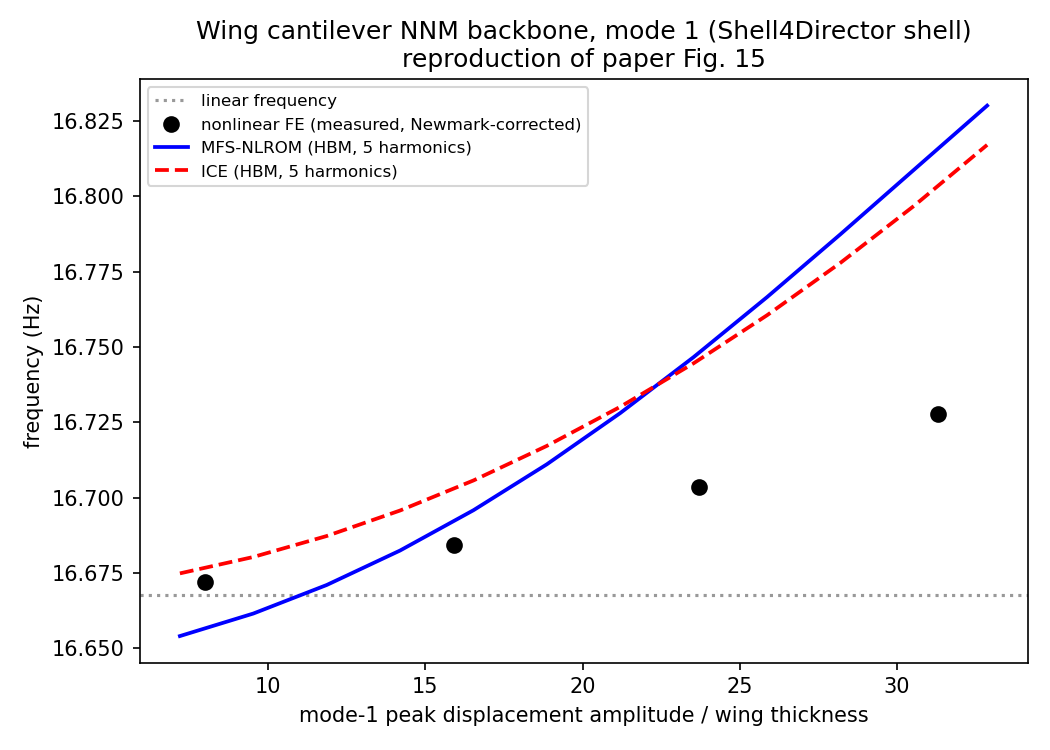
\includegraphics[width=0.6\linewidth]{figures/ch14r/mfs_wing_backbone.png}
\caption{Backbone of mode 1 of the shell wing: harmonic balance with five harmonics for the reduced models, free vibration from static equilibria for the full-order model. Plot of the reproduction report.}\label{fig:vf-mfs-wback}
\end{figure}

The solid wing model gives held-out $R^2$ of $0.780$ (surrogate, thin-plate spline) and $1.000$ (polynomial), a tip sweep of $0.9987$ and $1.0000$, and free decay of $0.9646$ and $1.0000$; its finite element reference fails to converge at large amplitude, so only one of three backbone points and a truncated window of case~(b) could be compared. The solid results are therefore secondary and are not used as evidence.

\subsection*{Comparison with the publication}

\begin{table}[tbp]
\centering\footnotesize
\caption{Claims of \citet{he2023mfsnlrom} and the outcome of the reproduction.}\label{tab:vf-mfs-cmp}
\begin{tabularx}{\linewidth}{@{}>{\raggedright\arraybackslash}p{4.1cm} >{\raggedright\arraybackslash}X >{\raggedright\arraybackslash}p{2.3cm}@{}}
\toprule
Claim & This work & Outcome\\
\midrule
Linear modes of the beam (Fig.~4) & within $0.15\,\%$ & reproduced\\
Nonlinear-force surfaces (Fig.~5) & axis ranges and shape match; training points unpublished & reproduced (shape)\\
Static accuracy by kernel (Table~2) & MQ and ICE agree; ranking of other kernels differs & partly\\
Pressure sweep and speed ordering (Fig.~6, Table~4) & $R^2=1.0000$; MFS $\gg$ ICE $\gg$ FE & reproduced\\
Free decay (Fig.~7, Table~3) & $R^2=0.990$--$0.997$ (publication 0.984); ICE failure ($-0.63$) not seen & reproduced; ICE failure not\\
Sample-size sensitivity (Fig.~8) & saturates near $N=10n$ & reproduced\\
Backbone (Fig.~9) & error $<1\,\%$ over a $22\,\%$ hardening & reproduced\\
Wing static, dynamic, backbone (Figs.~12, 15) & shell: $R^2=1.0000$, $0.9999$, error $\le0.53\,\%$ & reproduced on the shell\\
Hammer test (Figs.~13, 14) & measured signals cannot be recovered from the publication & not reproduced\\
\bottomrule
\end{tabularx}
\end{table}

\subsection*{What was not reproduced, and why}

The equations for the training-load scaling and the time-integration scheme of the publication did not survive text extraction from the PDF. The load scaling is structurally confirmed by the appendix of the publication, but its iterative calibration loop is not implemented; a fixed target-fraction range tuned to the axes of its Fig.~5 is used instead, and the time-integration scheme is a reconstruction that diverges on the flat beam, which is why a Newton solve of the same relation is used. The publication states no damping ratio, so $1\,\%$ modal Rayleigh damping is assumed in every dynamic case. The full-order backbone is obtained by free vibration and period measurement, not by the publication's multi-harmonic-balance solver on the full model. The wing planform is digitised, its frequencies lie $11$--$16\,\%$ from the publication's, and its training sizes are reduced. Both reduced models are valid only inside their training range, and the publication's hammer test cannot be rebuilt. Finally, the polynomial baseline matches or exceeds the surrogate in accuracy on these smooth, weakly nonlinear problems, so the benefit measured here is speed and generality, not accuracy.

An early failure of the flat-beam run (sweep $R^2=0.54$, free-decay $R^2=-1.00$, overflow of the baseline) came from the author's driver, which scanned the mode-shape peaks over rotation degrees of freedom and so made the training amplitudes 13 to 72 times too small. After the correction the sweep gives $R^2=1.000$ for both models; the sample-size curve at $N=9$ changed from 0.995 to 0.844 and the backbone span from $79.0$--$79.3$ to $80.6$--$96.3$~Hz.
